\section{Contemporary history and usage.} \label{now-history}

Less than an hour after Hofmann administered himself with the dose, it was clear that LSD was responsible for his anomalous state. With help from his assistant, he went back home by bike through a wavy landscape. Laying on the couch, his surroundings turned grotesque. His neighbour, who had brought some milk, had become an evil witch. He was terrorized by the thought that his experiment could leave his family fatherless. When the physician arrived, he gave no other advice than to wait it out, as his vitals were correct. Right guess, as he was able to descend from that gruesome scenario and enjoy the residual sinesthesias and caleidoscopic imagery. The next day he found himself as fresh as ever, remembering the whole experience.

Hofmann saw in LSD a drug of enormous importance in pharmacology, neurology and, mainly, psychiatry. He wouldn't have ever anticipated that it would be used in a recreational manner after what he lived through.

After informing his supervisor, Sandoz's pharmacological deparment started studying the tolerance and toxicity of the substance. The first animal tests displayed cats which observed apparently nothing and instead of attacking mice, looked at them in awe. Spiders built more efficient webs on low doses, but very poor ones at higher doses. When introduced into a community of chimpanzees, even if only a small subset of them took it, the whole group entered conflict due to them not following the hierarchical laws of their tribe.

With LSD's safety on humans assured, Sandoz started commercializing it as an experimental pharmaceutical: \textit{Delysid}. Among its uses was also mentioned self-experimentation from the psychiatrist to gain perspective on the internal emotion on their patients, as the experience served as a model for different disorders.

\subsection{Psychedelic therapy, art and recreation, prohibition.}

LSD doesn't act as a medicine \textit{per se}, that is, it doesn't --- as far as we know --- fix any chemical imbalance as an antidepressant would. However, given the peculiar effects it produces on conscioussness, its uses as an auxiliar pharmaceutical in psychotherapy and psychoanalysis have been very abundant. Because it takes the user's current internal state to its extreme, it's a very useful tool to liberate repressed material, making it efficient for treating trauma. Furthermore, because it dissolves the border that separates the \textit{you} from the \textit{I}, it facilitates the detachment from ego-centered problems. It has also been used in terminal cancer patients who develop too much tolerance to analgesics, although this poses ethical questions. The dissociation from the body prevents the pain from penetrating into conscioussness and offers the courage to face one's death. This use requires special supervision and preparation, being useful to have a psychotherapist or a religious figure guiding the experience. The famous writer Aldous Huxley asked his wife to be injected with 100 microgram doses in his deathbed, multiple times if necessary.

On the early 60s LSD becomes widespread on the West, with a notable influence on american society which was accompanied casual or causally by the birth of the hippie movement. Doctor Timothy Leary from University of Harvard was a very relevant figure in the difussion of LSD through the United States. He tested it on members of the clergy, convicts and artists, although his works quickly lost their scientific character and he was expelled from university. Turned to hinduism, he became one of the leaders of the hippie movement. With the neverending mantra of \enquote{Turn on, tune in, drop out}, he encouraged the youth to consume LSD (\textit{turn on}) to explore their inner worlds (\textit{tune in}) and finally detach from bourgeoisie life, studies, work and every other chain through the chant \enquote{\textit{drop out}} (Figure \ref{albums}).

\begin{figure}[H]
	\centering
	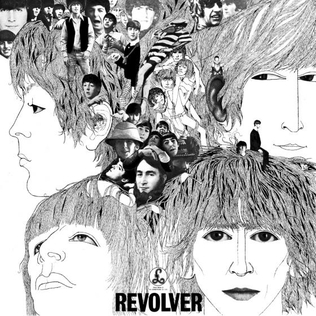
\includegraphics[height=.2\textheight]{media/10-revolver.jpg}
	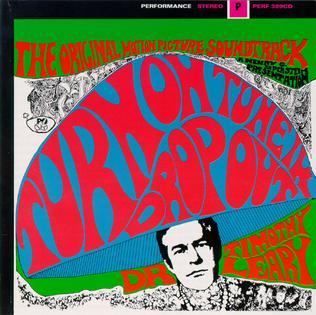
\includegraphics[height=.2\textheight]{media/10-leary.jpg}
	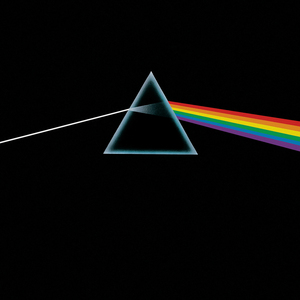
\includegraphics[height=.2\textheight]{media/10-dsotm.png}
	\caption{Covers of the albums \textit{Revolver} (The Beatles), \textit{Turn On, Tune In, Drop Out} (Timothy Leary) and \textit{The Dark Side of the Moon} (Pink Floyd), very influenced by LSD.}
	\label{albums}
\end{figure}

This subversion of the traditional structures was an uprising that challenged --- reminiscent to the chimpanzees that lost their hierarchical structure --- every social and political authority. Dr. Leary was arrested in Kabul and imprisoned for drug possesion. In 1976, now free, he worked on topics like the relationship between the CNS and interstellar space.

LSD followed a path similar to mescaline's: it started out as a chemical compound of interest in scientific and psychiatric groups and it sneaked among intellectuals. The aesthetic and introspective experiences it induced freed up the artists' creative process. Every work created after the use of LSD and other psychotropes like mescaline or psylocibin entered the realm of psychedelic art. The book \textit{Psychedelic art} contains an excellent collection of this genre.

In music, groups as popular as The Beatles were marked by this substance. Albums like \textit{Revolver} or \textit{Sgt. Pepper’s Lonely Hearts Club Band} and songs like \textit{Lucy in the Sky with Diamonds} (a title which is now used as an alias for this drug) received a deep aesthetic influence from LSD. Overall, contemporary bands like Pink Floyd, Jefferson Airplane and The Grateful Dead conceived the \textit{psychedelic rock} genre.

LSD also entered the common people. Hofmann anticipated some curiosity from artists and intellectuals, but he never thought his creation could be used as a common intoxicant, and this use produced some incidents. Clinical and university experiments with the drug stopped being shared on scientific papers and started being presented to everyone in magazines and newspapers, where conclusions were often exagerated. Reports about this drugs weren't done in third person anymore, instead the journalists consumed it and later wrote their experiences. On american markets, books commenting on LSD's effects appeared, and it was common for them to be elated.

All this literature implanted a wrong idea in popular culture: that just using this medicine was enough to achieve miraculous effects. Under such conception, the reign of self-experimentation begun. The sixties, with an existential crisis in american society, the complete legality of the substance and Sandoz's patents expiration, made LSD omnipresent. As it was to be expected, popular experiences were more similar to the firsts ones from Albert Hofmann. \enquote{Bad trips}, disorientation and panic were a habitual product of self-experimentation, sometimes leading to accidents and crimes.

Between 1964 and 1966, the controversy with LSD was evident, with enthusiasts saying it was a magical substance and others who pointed out the accidents and crimes that were comitted under its effects. Sandoz suffered massive sues on the properties of the substance. Finally, on August of 1965, they stopped publically producing and exporting Delysid. In exchange, they offered it to qualified researchers around the world, with both technical and financial assistance. In addition to the detailed description in \textit{Catalogue of Literature on Delysid}, the improper use of the substance was quite inhibited.

Sandoz couldn't however control every possible exception. The wrong ideas in place and the total absence of legislation forced Sandoz to cease production of LSD and similar hallucinogens like psilocybin. UNO's \textit{Convention on Psychotropic Substances} and America's \textit{Controlled Substances Act} not only forbade possesion and distribution, but also discarded any therapeutic use of the substance. Its association with an \enquote{insanity drug} disuaded psychiatrists from using it. Like a tragic family curse, LSD was condemned to ostracism just as was ergot three centuries before.

The decline on LSD's use has notably affected its production. In psychiatric and neurobiological studies it has been substituted by substances like psylocibin (found on hallucinogenic mushrooms), not only because of its similarities in pharmacology and effects, but also because its more brief time of actions facilitates its study. As an illegal drug it has also been replaced by cannabis derivatives like hashish and synthetic drugs like heroin and amphetamines, usually being more toxic than what they substitute.

\subsection{LSD's risks.}

Current legislation doesn't attribute any therapeutic usage to LSD. There are opposing opinions which argue that there's no danger if used in a professional setting. Some even say that the existing danger outside these environments is more related to the secrecy than to the substance itself. It can't be negated that LSD usage is linked to a series of risks that must be known whether it's used in a professional setting with medical supervision or not.

The disorientation intrinsic to every LSD experiment makes it impossible to discard crisis episodes, it doesn't matter how much it can be minimized through preparation. Worst case scenario, the psychosis will inhibit the individual's risk perception, producing fatal accidents. On the other hand, an experience with mortiferous visions can end in suicide. Even if they're not common cases, they must serve as a warning. Frank Olson, an american physician, consumed high doses of LSD without his knowledge. He killed himself jumping out of a window. He had been a victim in pharmacological experiments from the US army. It wouldn't be until 15 years later that, with the relevation of project MK Ultra, CIA's director William Collby and US president Gerald Ford presented their apologies to the family.

It's also important to analyse whether LSD is the optimal pharmaceutical for the patient's wellbeing, administering it just in the right cases. Because LSD intensifies the current mental state, offering it to a patient with the intention of curing a bad mood can be very harmful. It shouldn't either be used in unstable personalities, like those prone to psychosis. This, in general, includes young people.

A commentary on the personal use LSD receives is necessary. There exists an intrinsic problem in the personal use of any drug. If by definition they act on the nervous system, affecting emotion and perception --- and our judgement is precisely based on these faculties --- then our decision making will be compromised, including the decision to consume the drug. Ideas accepted or rejected in a state of consciousness may not be in another one even when previous planning is carefully made. This matter poses a debate on the relationship between free will and the nervous system, but we won't touch on it.

It's impossible to do a scientific study on the personal use of LSD. If we were to establish a controlled environment and follow each individual's progress, the use would stop being personal. We are then dependent on the \enquote{popular wisdom} communicated by journalists and individuals like Albert Hofmann himself. For example, in many sources the concept of \textit{set and setting} is mentioned as what determines whether the feelings during an experience will be mainly good or bad. The set of internal factors like previous mood and expectations is what we call \textit{set}. Whereas \textit{setting} describes external factors like the environment's character, its illumination, its ambiance noise or the people present. The importance of someone trusted who can offer emotional support or call for medical assistance is also mentioned. The use of a correct dosage is stressed, being recommended to start on very low doses and write a history with the effects of each one.

Finally, we need to remember that LSD is illegal, and hence the dark market is the only option available for its purchase. This poses risks completely different from the pharmacological ones. Because they're not regulated, the purity of clandestine products is unknown, and it's common to find them contaminated by other substances. Apart from purity, there's the problem of dosage: even if the measure is included in micrograms (also called \enquote{\textit{gammas}}), it can be altered. Given the huge difference between doses of 25, 100 and 600 micrograms of LSD, the uncertainty when consuming an underground product makes bad experiences much more common.

\newpage
